\chapter{\oracle: \EN{.MSB-files}\RU{.MSB-файлы}}
\index{\oracle}
\EN{\epigraph{When working toward the solution of a problem, it always helps if you know the answer.}{Murphy's Laws, Rule of Accuracy}}
\RU{\epigraph{Работая над решением задачи, всегда полезно знать ответ.}{Законы Мерфи, правило точности}}

\RU{Это бинарный файл содержащий сообщения об ошибках вместе с их номерами.}
\EN{This is a binary file containing error messages with corresponding numbers.}
\RU{Давайте попробуем понять его формат и найти способ распаковать его}\EN{Let's try to understand 
its format and find a way to unpack it}.

\RU{В \oracle имеются файлы с сообщениями об ошибках в текстовом виде, так что мы можем сравнивать файлы:
текстовый и запакованный бинарный}\EN{There are \oracle error message files in text form, 
so we can compare text and packed binary files}
\footnote{\EN{Text files are exist in \oracle not for every .MSB file, so that's why I worked on its file format}
\RU{Текстовые файлы в \oracle имеются не для каждого .MSB-файла, вот почему я работал над его форматом}}.

\RU{Это начало файла}\EN{This is the beginning of} ORAUS.MSG \RU{без ненужных комментариев}\EN{text files 
with irrelevant comments stripped}:

\begin{lstlisting}[caption=\RU{Начало файла}\EN{Beginning of} ORAUS.MSG \RU{без комментариев}\EN{file without comments}]
00000, 00000, "normal, successful completion"
00001, 00000, "unique constraint (%s.%s) violated"
00017, 00000, "session requested to set trace event"
00018, 00000, "maximum number of sessions exceeded"
00019, 00000, "maximum number of session licenses exceeded"
00020, 00000, "maximum number of processes (%s) exceeded"
00021, 00000, "session attached to some other process; cannot switch session"
00022, 00000, "invalid session ID; access denied"
00023, 00000, "session references process private memory; cannot detach session"
00024, 00000, "logins from more than one process not allowed in single-process mode"
00025, 00000, "failed to allocate %s"
00026, 00000, "missing or invalid session ID"
00027, 00000, "cannot kill current session"
00028, 00000, "your session has been killed"
00029, 00000, "session is not a user session"
00030, 00000, "User session ID does not exist."
00031, 00000, "session marked for kill"
...
\end{lstlisting}

\RU{Первое число это код ошибки}\EN{The first number is error code}.
\RU{Второе это может быть дополнительные флаги, но я не уверен}\EN{The second is maybe some additional flags, 
but I'm not sure}.

\clearpage
\RU{Давайте откроем бинарный файл}\EN{Now let's open} ORAUS.MSB 
\RU{и найдем эти текстовые строки}\EN{binary file and find these text strings}. 
\RU{И вот они}\EN{And there are}:

\begin{figure}[H]
\centering
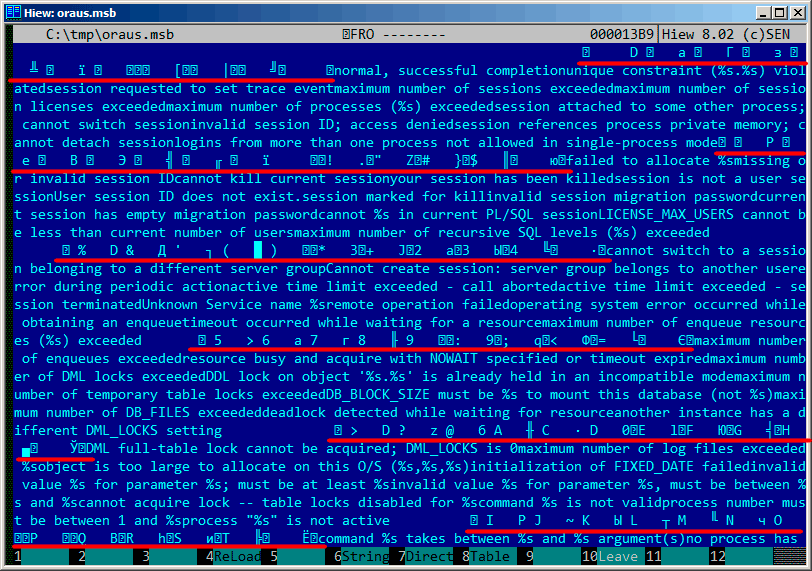
\includegraphics[scale=\FigScale]{ff/Oracle_MSB/1.png}
\caption{Hiew: \RU{первый блок}\EN{first block}}
\label{fig:oracle_MSB_1}
\end{figure}

\RU{Мы видим текстовые строки (включая те, с которых начинается файл ORAUS.MSG) перемежаемые с какими-то
бинарными значениями}\EN{We see the text strings (including those with which ORAUS.MSG file started) 
interleaved with some binary values}.
\RU{Мы можем довольно быстро обнаружить что главная часть бинарного файла поделена на блоки размером 0x200 (512)
байт}\EN{By quick investigation, we can see that main part of binary file is divided by blocks of 
size 0x200 (512) bytes}.

\clearpage
\RU{Посмотрим содержимое первого блока}\EN{Let's see contents of the first block}:

\begin{figure}[H]
\centering
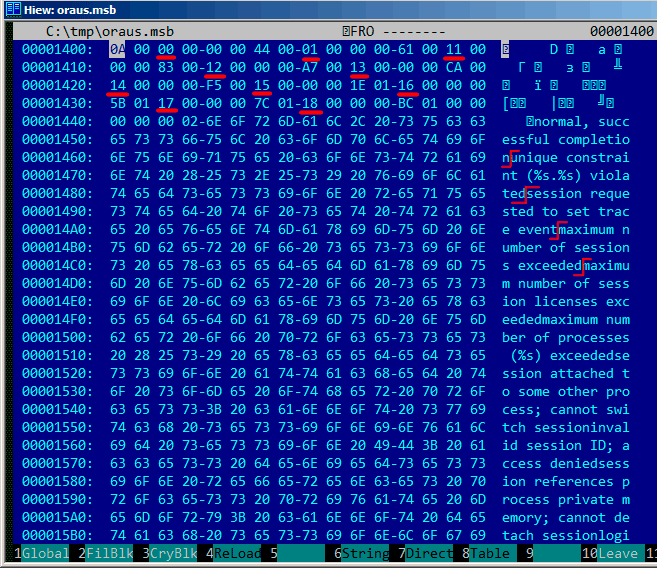
\includegraphics[scale=\FigScale]{ff/Oracle_MSB/2.png}
\caption{Hiew: \RU{первый блок}\EN{first block}}
\label{fig:oracle_MSB_2}
\end{figure}

\RU{Мы видим тексты первых сообщений об ошибках}\EN{Here we see texts of first messages errors}.
\RU{Что мы видим еще, так это то, что здесь нет нулевых байтов между сообщениями}\EN{What we also see is 
that there are no zero bytes between error messages}.
\RU{Это значит что это не оканчивающиеся нулем Си-строки}\EN{This mean, these are not zero-terminated C-strings}.
\RU{Как следствие, длина каждого сообщения об ошибке должна быть как-то закодирована}\EN{As a consequence, 
a length of each error message must be coded somehow}.
\RU{Попробуем также найти номера ошибок}\EN{Let's also try to find error numbers}.
\RU{Файл}\EN{The} ORAUS.MSG \RU{начинается с таких}\EN{files started with these}: 
0, 1, 17 (0x11), 18 (0x12), 19 (0x13), 20 (0x14), 21 (0x15), 22 (0x16), 23 (0x17), 24 (0x18)...
\RU{Я нашел эти числа в начале блока и отметил их красными линиями}\EN{I found these numbers in the beginning 
of block and marked them with red lines}.
\RU{Период между кодами ошибок 6 байт}\EN{The period between error codes is 6 bytes}.
\RU{Это значит, здесь наверное 6 байт информации выделено для каждого сообщения об ошибке}\EN{This mean, 
there are probably 6 bytes of information allocated for each error message}.

\RU{Первое 16-битное значение (здесь 0xA или 10) означает количество сообщений в блоке: я проверил это
глядя на другие блоки}\EN{The first 16-bit value (0xA here or 10), mean number of messages in each block: 
I checked this by investigating other blocks}.
\RU{Действительно: сообщения об ошибках имеют произвольный размер}\EN{Indeed: error messages has arbitrary size}. 
\RU{Некоторые длиннее, некоторые короче}\EN{Some are longer, some are shorter}. 
\RU{Но длина блока всегда фиксирована, следовательно, никогда не знаешь, сколько сообщений можно запаковать
в каждый блок}\EN{But block size is always fixed, hence,
you never know how many text messages can be packed in each block}.

\RU{Как я уже отметил, так как это не оканчивающиеся нулем Си-строки, длина строки должна быть закодирована
где-то}\EN{As I already noted, since this is not zero-terminating C-strings, 
a string size should be encoded somewhere}.
\RU{Длина первой строки}\EN{The size of the first string} ``normal, successful completion'' \RU{это}\EN{is} 
29 (0x1D) \RU{байт}\EN{bytes}.
\RU{Длина второй строки}\EN{The size of the second string} ``unique constraint (\%s.\%s) violated'' 
\RU{это}\EN{is} 34 (0x22) \RU{байт}\EN{bytes}.
\RU{Мы не можем отыскать этих значений}\EN{We can't find these values} (0x1D \OrENRU/\AndENRU 0x22) 
\RU{в блоке}\EN{in the block}.

\RU{А вот еще кое-что}\EN{There is also another thing}.
\oracle \RU{должен как-то определять позицию строки, которую он должен загрузить, верно}\EN{should somehow 
determine position in block of the string it needs to load, right}?
\RU{Первая строка}\EN{The first string} ``normal, successful completion'' \RU{начинается с позиции}\EN{is started 
at the position of} 0x1444 (\RU{если считать с начала бинарного файла}\EN{if to count starting at the binary file}) \RU{или с}\EN{or at} 0x44 (\RU{от начала блока}\EN{starting at the block begin}).
\RU{Вторая строка}\EN{The second string} ``unique constraint (\%s.\%s) violated'' 
\RU{начинается с позиции}\EN{is started at the position of} 0x1461 (\RU{от начала файла}\EN{from the
file start}) \RU{или с}\EN{or at} 0x61 (\RU{считая с начала блока}\EN{starting at the block begin}).
\RU{Эти числа}\EN{These} (0x44 \AndENRU 0x61) \RU{нам знакомы}\EN{are familiar numbers}! 
\RU{Мы их можем легко отыскать в начале блока}\EN{We can clearly see them at the block start}.

\RU{Так что, каждый 6-байтный блок это}\EN{So, each 6-byte block is}:

\begin{itemize}
\item 16-\RU{битный номер ошибки}\EN{bit error number}; 
\item 16-\RU{битный ноль (может быть, дополнительные флаги}\EN{bit zero (may be additional flags)}; 
\item 16-\RU{битная начальная позиция текстовой строки внутри текущего блока}\EN{bit starting position of 
the text string within the current block}.
\end{itemize}

\RU{Я могу быстро проверить остальные значения чтобы удостовериться в своей правоте}\EN{I can quickly check 
other values and be sure I'm right}.
\RU{И здесь еще последний ``пустой'' 6-байтный блок с нулевым номером ошибки и начальной позицией за последним
символом последнего сообщения об ошибке.}\EN{And there are also the last ``dummy'' 6-byte block 
with zero error number and starting position beyond the last error message last character.}
\RU{Может быть именно так и определяется длина сообщения}\EN{Probably that's how text message length is 
determined}?
\RU{Мы просто перебираем 6-байтные блоки в поисках нужного номера ошибки, затем
мы узнаем позицию текстоврой строки, затем мы узнаем позицию следующей текстовой строки глядя на
следующий 6-байтный блок!}\EN{We just enumerate 6-byte blocks to find error number
we need, then we get text string position, then we get position of the text string by looking onto next
6-byte block!}
\RU{Так мы определяем границы строки}\EN{Thus we determine string boundaries}!
\RU{Этот метод позволяет сэкономить место в файле не записывая длину строки}\EN{This method allows to 
save a space by not saving text string size in the file}!
\RU{Нельзя сказать, что экономия большая, но это интересный трюк}\EN{I cannot say it saves a lot, 
but it's a clever trick}.

\clearpage
\RU{Вернемся к заголовку .MSB-файла}\EN{Let's back to the header of .MSB-file}:

\begin{figure}[H]
\centering
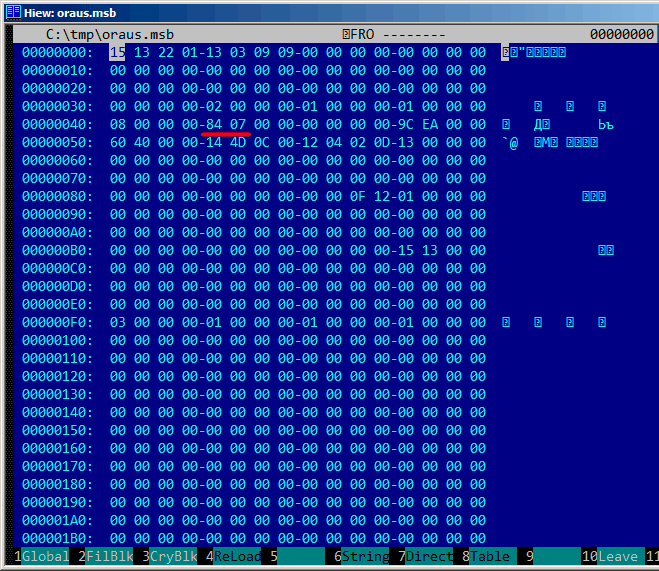
\includegraphics[scale=\FigScale]{ff/Oracle_MSB/3.png}
\caption{Hiew: \RU{заголовок файла}\EN{file header}}
\label{fig:oracle_MSB_3}
\end{figure}

\RU{Я быстро нашел количество блоков (отмечено красным)}\EN{I quickly found number of blocks in file 
(marked by red)}.
\RU{Я проверил другие .MSB-файлы и это справедливо для всех}\EN{I checked other .MSB-files and that's true 
for any}.
\RU{Здесь есть много других значений, но я не разбирался с ними, так как моя задача (утилита для распаковки)
уже решена.}
\EN{There are a lot of other values, but I didn't investigate them, since by job (unpacking utility) was done.}
\RU{А если бы я писал запаковщик .MSB-файлов, тогда мне наверное пришлось бы понять, зачем нужны остальные.}
\EN{If I would write .MSB-file packer, I would probably need to understand other value meanings.}

\clearpage
\RU{Тут еще есть таблица после заголовка, вероятно, содержащая 16-битные значения}\EN{There is also a 
table came after header which probably contain 16-bit values}:

\begin{figure}[H]
\centering
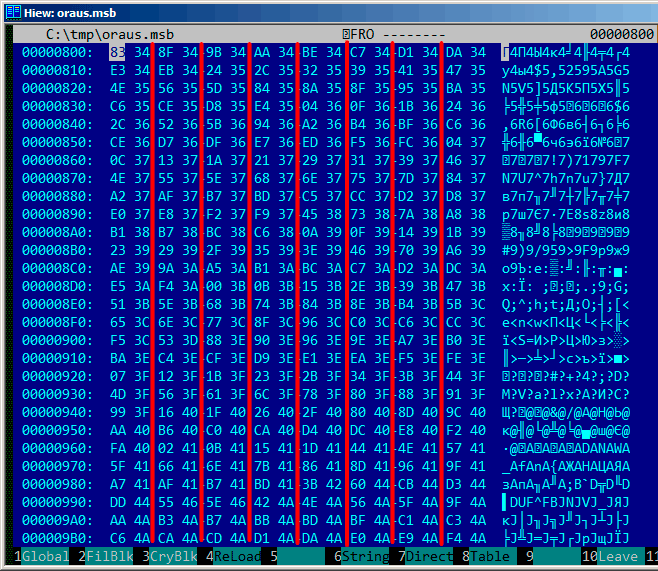
\includegraphics[scale=\FigScale]{ff/Oracle_MSB/4.png}
\caption{Hiew: \RU{таблица }last\_errnos\EN{ table}}
\label{fig:oracle_MSB_4}
\end{figure}

\RU{Их длина может быть определена визуально (я нарисовал красных линий)}\EN{Their size can be determined 
visually (I draw red lines)}.
\RU{Когда я сдампил эти значения, я обнаружил, что каждое 16-битное число это последний код ошибки для
каждого блока}\EN{When I'm dumping these values, I found that each 16-bit number is a last error 
code for each block}.\\
\\
\RU{Так вот как \oracle быстро находит сообщение об ошибке}\EN{So that's how \oracle quickly finds error message}:

\begin{itemize}
\item \RU{загружает таблицу, которую я назвал}\EN{load a table I called} last\_errnos 
(\RU{содержащую последний номер ошибки для каждого блока}\EN{containing last error number for each block});
\item \RU{находит блок содержающий код ошибки, полагая что все коды ошибок увеличиваются и внутри каждого блока
и также в файле}\EN{find a block containing error code we need, assuming all error codes 
increasing across each block and the file as well};
\item \RU{загружает соответствующий блок}\EN{load specific block};
\item \RU{перебирает 6-байтные структуры, пока не найдется соответсвующий номер ошибки}\EN{enumerate 6-byte 
structures until specific error number is found};
\item \RU{находит позицию первого символа из текущего 6-байтного блока}\EN{get a position of the first 
character from current 6-byte block};
\item \RU{находит позицию последнего символа из следующего 6-байтного блока}\EN{get a position of the last 
character from the next 6-byte block};
\item \RU{загружает все символы сообщения в этих пределах}\EN{load all characters from message in this range}.
\end{itemize}

\RU{Это программа на Си которую я написал для распаковки .MSB-файлов}\EN{This is C-program I wrote which 
unpacks .MSB-files}:
\url{http://go.yurichev.com/17213}.

\RU{И еще два файла которые я использовал в этом примере}\EN{There are also two files I used in the example} 
(\oracle 11.1.0.6):
\url{http://go.yurichev.com/17214},
\url{http://go.yurichev.com/17215}.

\section{\RU{Вывод}\EN{Summary}}

\RU{Этот метод наверное слишком олд-скульный для современных компьютеров}\EN{The method is probably too 
old-school for modern computers}.
\RU{Возможно, формат этого файла был разработан в середине 1980-х кем-то, кто программировал для мейнфреймов,
учитывая экономию памяти и места на дисках}\EN{Supposedly, this file format was developed in the mid-80's by 
someone who also coded for \IT{big iron} with
memory/disk space economy in mind}.
\RU{Тем не менее, это интересная (хотя и простая) задача на разбор проприетарного формата файла без
заглядывания в код \oracle}\EN{Nevertheless, it was an interesting and yet easy task 
to understand proprietary file format without looking into \oracle code}.
